\documentclass[12pt, a4paper]{article}
\usepackage[lmargin =0.5 in, 
rmargin=0.5in, 
tmargin=1in,
bmargin=0.5in]{geometry}
\geometry{letterpaper}
\usepackage{tikz-cd}
\usepackage{amsmath}
\usepackage{amssymb}
\usepackage{blindtext}
\usepackage{titlesec}
\usepackage{enumitem}
\usepackage{fancyhdr}
\usepackage{amsthm}
\usepackage{graphicx}
\usepackage{cool}
\usepackage{thmtools}
\usepackage{hyperref}
\usepackage{pythonhighlight}
\graphicspath{ }					%path to an image

%-------- sexy font ------------%
%\usepackage{libertine}
%\usepackage{libertinust1math}

%\usepackage{mlmodern}				% very nice and classic
%\usepackage[utopia]{mathdesign}
%\usepackage[T1]{fontenc}


\usepackage{mlmodern}
\usepackage{eulervm}
%\usepackage{tgtermes} 				%times new roman
%-------- sexy font ------------%


% Problem Styles
%====================================================================%


\newtheorem{problem}{Problem}


\theoremstyle{definition}
\newtheorem{thm}{Theorem}
\newtheorem{lemma}{Lemma}
\newtheorem{prop}{Proposition}
\newtheorem{cor}{Corollary}
\newtheorem{fact}{Fact}
\newtheorem{defn}{Definition}
\newtheorem{example}{Example}
\newtheorem{question}{Question}

\newtheorem{manualprobleminner}{Problem}

\newenvironment{manualproblem}[1]{%
	\renewcommand\themanualprobleminner{#1}%
	\manualprobleminner
}{\endmanualprobleminner}

\newcommand{\penum}{ \begin{enumerate}[label=\bf(\alph*), leftmargin=0pt]}
	\newcommand{\epenum}{ \end{enumerate} }

% Math fonts shortcuts
%====================================================================%

\newcommand{\ring}{\mathcal{R}}
\newcommand{\N}{\mathbb{N}}                           % Natural numbers
\newcommand{\Z}{\mathbb{Z}}                           % Integers
\newcommand{\R}{\mathbb{R}}                           % Real numbers
\newcommand{\C}{\mathbb{C}}                           % Complex numbers
\newcommand{\F}{\mathbb{F}}                           % Arbitrary field
\newcommand{\Q}{\mathbb{Q}}                           % Arbitrary field
\newcommand{\PP}{\mathcal{P}}                         % Partition
\newcommand{\M}{\mathcal{M}}                         % Mathcal M
\newcommand{\eL}{\mathcal{L}}                         % Mathcal L
\newcommand{\T}{\mathbb{T}}                         % Mathcal T
\newcommand{\U}{\mathcal{U}}                         % Mathcal U\\
\newcommand{\V}{\mathcal{V}}                         % Mathcal V

% symbol shortcuts
%====================================================================%

\newcommand{\bd}{\partial}
\newcommand{\grad}{\nabla}
\newcommand{\lam}{\lambda}
\newcommand{\imp}{\implies}
\newcommand{\all}{\forall}
\newcommand{\exs}{\exists}
\newcommand{\delt}{\delta}
\newcommand{\ep}{\varepsilon}
\newcommand{\ra}{\rightarrow}
\newcommand{\vph}{\varphi}

\newcommand{\ol}{\overline}
\newcommand{\f}{\frac}
\newcommand{\lf}{\lfrac}
\newcommand{\df}{\dfrac}

% bracketting shortcuts
%====================================================================%
\newcommand{\abs}[1]{\left| #1 \right|}
\newcommand{\babs}[1]{\Big|#1\Big|}
\newcommand{\bound}{\Big|}
\newcommand{\BB}[1]{\left(#1\right)}
\newcommand{\dd}{\mathrm{d}}
\newcommand{\artanh}{\mathrm{artanh}}
\newcommand{\Med}{\mathrm{Med}}
\newcommand{\Cov}{\mathrm{Cov}}
\newcommand{\Corr}{\mathrm{Corr}}
\newcommand{\tr}{\mathrm{tr}}
\newcommand{\Range}[1]{\mathrm{range}(#1)}
\newcommand{\Null}[1]{\mathrm{null}(#1)}
\newcommand{\lan}{\langle}
\newcommand{\ran}{\rangle}
\newcommand{\norm}[1]{\left\lVert#1\right\rVert}
\newcommand{\inn}[1]{\lan#1\ran}
\newcommand{\op}[1]{\operatorname{#1}}
\newcommand{\bmat}[1]{\begin{bmatrix}#1\end{bmatrix}}
\newcommand{\pmat}[1]{\begin{pmatrix}#1\end{pmatrix}}
\newcommand{\vmat}[1]{\begin{vmatrix}#1\end{vmatrix}}

\newcommand{\amogus}{{\bigcap}\kern-0.8em\raisebox{0.3ex}{$\subset$}}
\newcommand{\Note}{\textbf{Note: }}
\newcommand{\Aside}{{\bf Aside: }}
%restriction
%\newcommand{\op}[1]{\operatorname{#1}}
%\newcommand{\done}{$$\mathcal{QED}$$}

%====================================================================%


\setlength{\parindent}{0pt}      	% No paragraph indentations
\pagestyle{fancy}
\fancyhf{}							% fancy header

\setcounter{secnumdepth}{0}			% sections are numbered but numbers do not appear
\setcounter{tocdepth}{2} 			% no subsubsections in toc

%template
%====================================================================%
%\begin{manualproblem}{1}
%Spivak.
%\end{manualproblem}

%\begin{proof}[Solution]
%\end{proof}

%----------- or -----------%

%\begin{problem} 		
%\end{problem}	

%\penum
%	\item
%\epenum
%====================================================================%


\newcommand{\Course}{MAT461}
\newcommand{\hwNumber}{1}

%preamble

\title{}
\author{A.N.}
\date{\today}
\lhead{\Course A\hwNumber}
\rhead{\thepage}
%\cfoot{\thepage}


%====================================================================%
\begin{document}



\begin{problem}
\end{problem}
A Galilean Transformation must be affine linear (Arnold pg 6), so $g$ must have the following form : 
$$g(x,t) = \bmat{A & B \\ C  & D} \bmat{x \\ t} + \bmat{b\\c }.$$ 
Since $g$ is Galilean, it must preserve the time interval. Suppose that we have two spacetime  points $(y,t_1), (y,t_2)$ so that $t( (x,t_1) -(y,t_2)  ) = t_1 - t_2$. We must also have that $t(g(x,t_1) - g(y, t_2)) = t_1 - t_2$. It follows that:
\begin{align*}t_1 - t_2 & = t \left( \bmat{A & B \\ C  & D} \bmat{x \\ t_1 } + \bmat{b\\c }  - \bmat{A & B \\ C  & D} \bmat{y \\ t_2} - \bmat{b\\c }\right)
	\\ & = t\left( \bmat{A x + t_1 B \\ C \cdot x + D t_1} - \bmat{A y + t_2 B \\ C \cdot y + D t_2} \right) 
	\\ & =C \cdot x + D t_1 - C y- D t_2.
\end{align*}
We wish for this to hold for all $x,y$  so we must have that $C = 0$ and $D = 1$. Fix a time $t$. Since $g$ preserves norms on simultaneous events, we must have that for any $(x,t), (y,t)$:
$$\norm{x- y} = \norm{g(x,t) - g(y,t)} = \norm{Ax - A y}.$$
Therefore $A$ must be an orthogonal matrix possibly depending on $t$. Relabeling we have that 
$$g(x,t) = \bmat{G_t & v \\ 0 & 1 } \bmat{x\\t} + \bmat{ \tilde{s} + vs \\ s}. $$ 
Where $\tilde{s}$ is chosen such that $\tilde{s} = b - vs$. Next we claim that for all $t$, $G_t = G$ for some $G\in O(3)$. We write for all $t$ that $G_t x = G_0x + y_t$ for some displacement vector $y_t$. The characterizing property of affine linear maps is that there exists some unique linear mapping $L$ so that for all $(x,t_1), (y,t_2)$, 
$$g(x,t_1) - g(y,t_2) = L \left((x,t_1) - (y,t_2) \right).$$
We apply this fact at $(x,t)$ and $(x,0)$:
$$L(0,t) = g(x,t) - g(x,0) = (y_t + tv , t).$$
Since the lefthand side is linear in $t$, the righthand side must be as well. Thus $y_t = ty$ for some $y$. We can write $$G_tx = G_0 x + ty.$$
Since $G_t,G_0$ preserve norms, both sides must have norms of $\norm{x}$. So 
$$\norm{x} = \norm{G_t x} = \norm{G_0 x + yt} = \norm{G_0x}.$$
The only way for this to hold for all $x,t$ is that $y=0$. So $G_t = G_0=G$. Therefore $$g(x,t) = \bmat{G & v \\ 0 & 1} \bmat{x \\ t} +  \bmat{\tilde{s} + vs \\ s}.$$
Note that the way $g(x,t)$ is written, it is the composition of a time translation, uniform motion, and a rigid motion. So $g = g_1\circ g_2 \circ g_3$. Suppose that there existed some other such transformations so that $g = h_1 \circ h_2 \circ h_3$. In coordinates, we have that
$$(t+s, Gx + \tilde{s} + v(t+s)) = (t + s^\prime , Hx + \tilde{s^\prime } + v^\prime (t+s^\prime)). \quad \quad (*)$$
It immediately follows that $s = s^\prime$. Taking $x=0$ gives us that 
$$\tilde{s} + v(t+s) = \tilde{s^\prime } + v^\prime(t+s).$$
Taking $t = -s$ gives us that $\tilde{s} = \tilde{s^\prime}$, and at $t = 0$ we have that $v= v^\prime$. It follows that $G = H$ since $(*)$ holds for all $x,t$. 
\newpage
\begin{problem}
\end{problem}
The following sketch is the phase portrait of the system given by potential $U(x)= -x^3(x-2)(x-4) $.
$$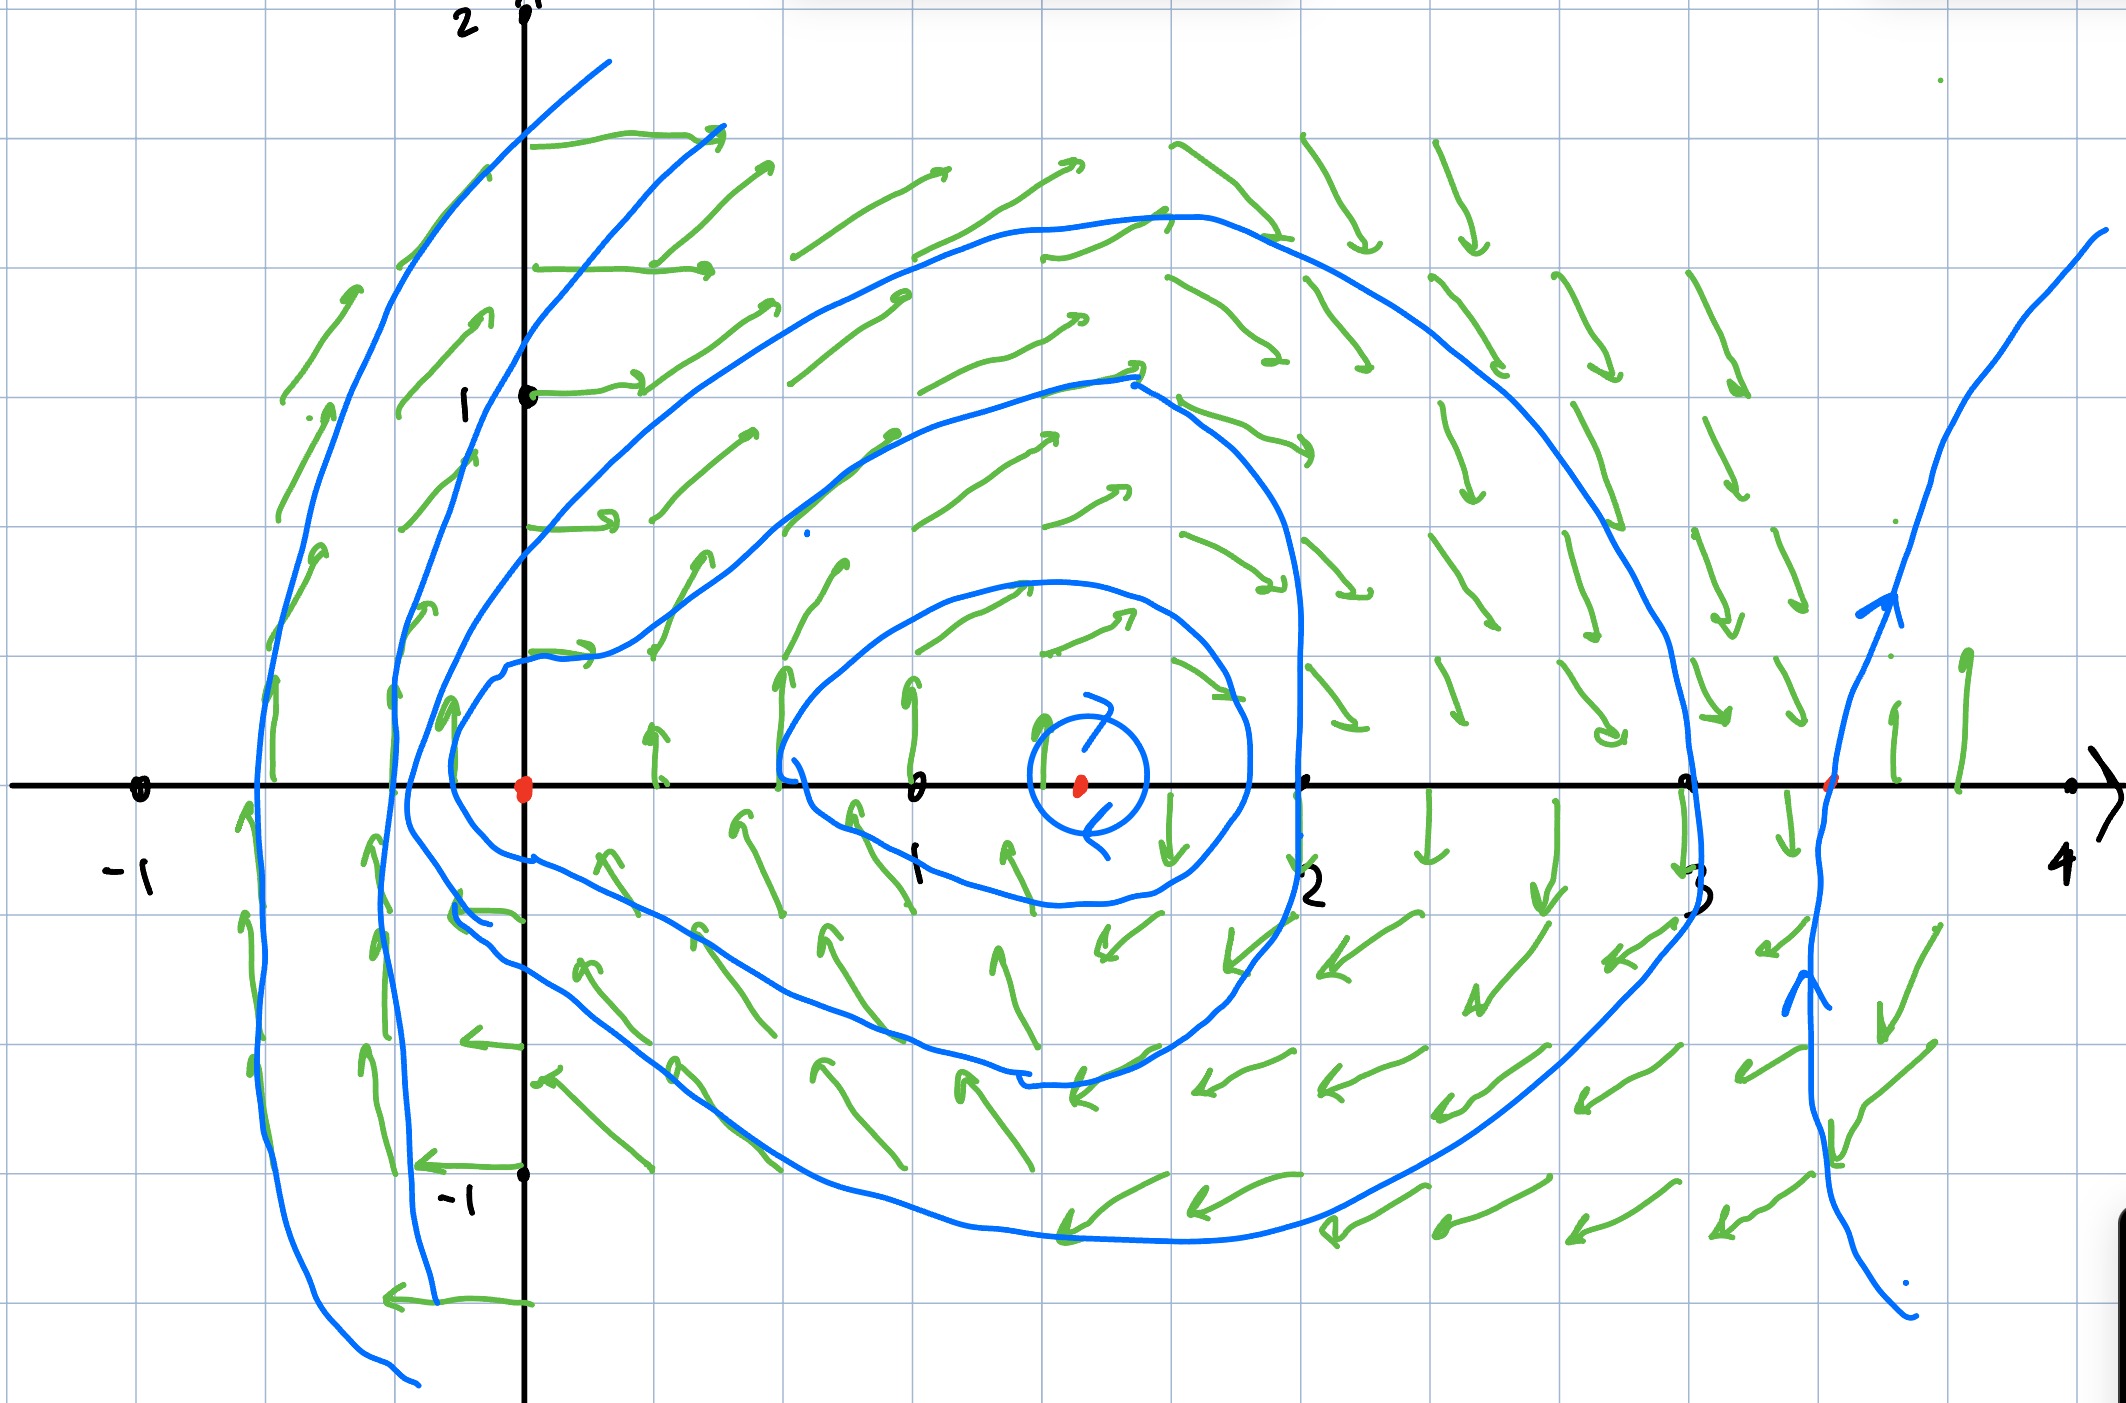
\includegraphics[width =\textwidth ]{mat461A1Q2.png}$$
The process to obtain the sketch is as follows: 
\begin{enumerate}
	\item Compute $f(x) = -\grad U(x)$:
	$$-\grad U(x) = x^2(5x^2-24x+24).$$
	\item Along the x-axis, at evenly spaced $x_i$ plot an vector of the form $(0, f(x_i))$. 
	\item Vary $y$ for fixed $x_i$, so that the $x$ component of our vector field changes. as we increase or decrease $y$. 
\end{enumerate}
Some observations of the system by glancing at the phase portrait
\begin{enumerate}
	\item Solutions near $x=0,y=0$ either exhibit periodic motion if slightly displaced to the right, but if the energy is sufficiently large the solutions will go off towards infinity. 
	\item Solutions near $x = 1.42$ with sufficiently low energy will have roughly periodic motion. If energy is too high they will escape the local minimum and go off towards infinity. 
	\item Solutions near $x = 3.38$ are extremely unstable. They tend to go off towards infinity. 
	\item Separatrix' shown in dotted red lines. Behavior of solution changes depending on which side of the separatrix a solution begins on. 
\end{enumerate}
\newpage
\begin{problem}
\end{problem}
The dynamics for 10 points is shown below:  
$$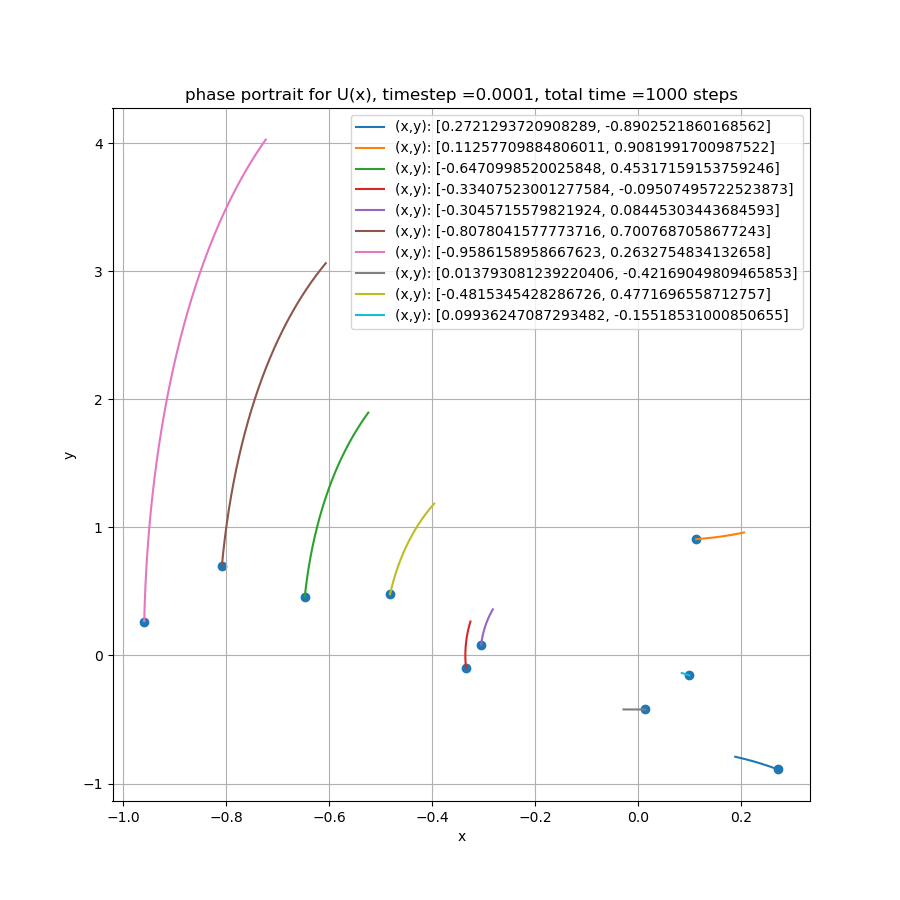
\includegraphics[width = 0.5 \textwidth]{mat461A1q31000 timesteps.png} 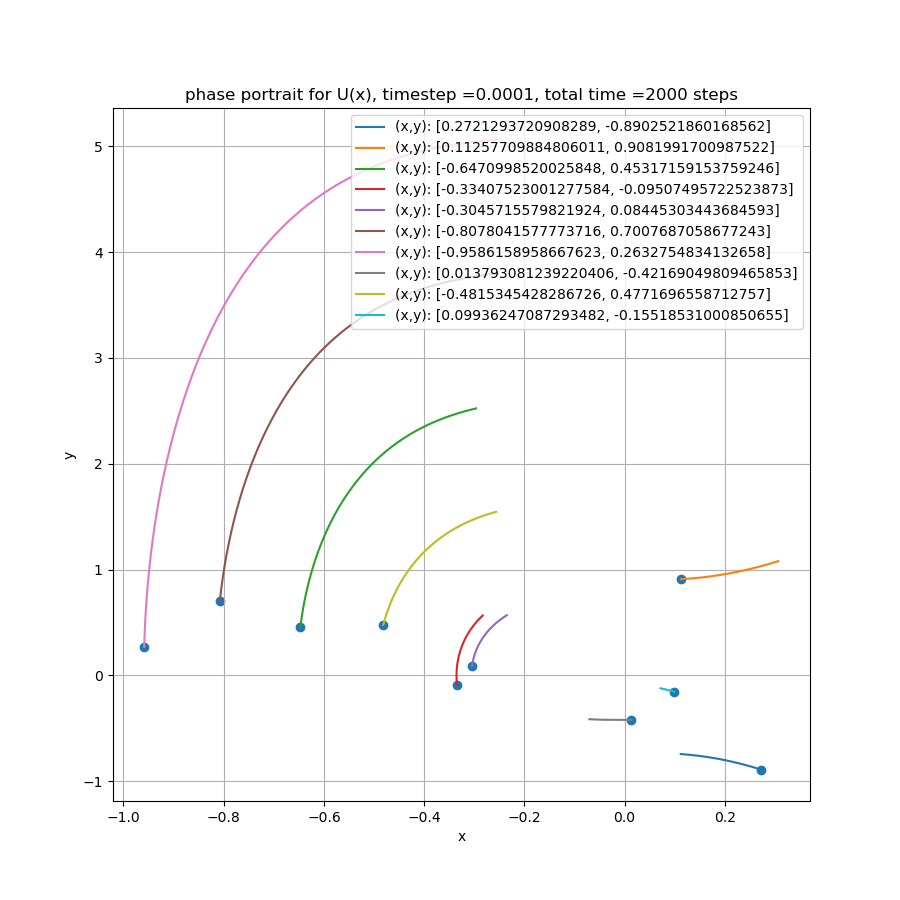
\includegraphics[width= 0.5 \textwidth]{mat461A1q32000 timesteps.png} $$ $$ 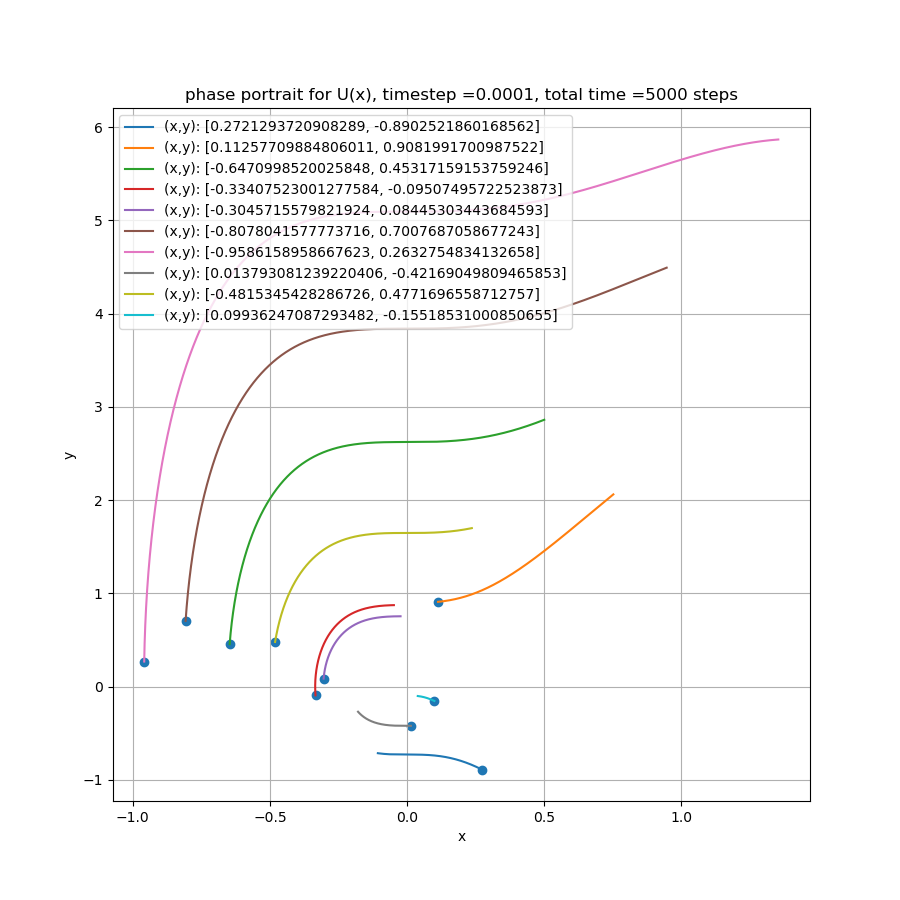
\includegraphics[width=0.5 \textwidth]{mat461A1q35000 timesteps.png} 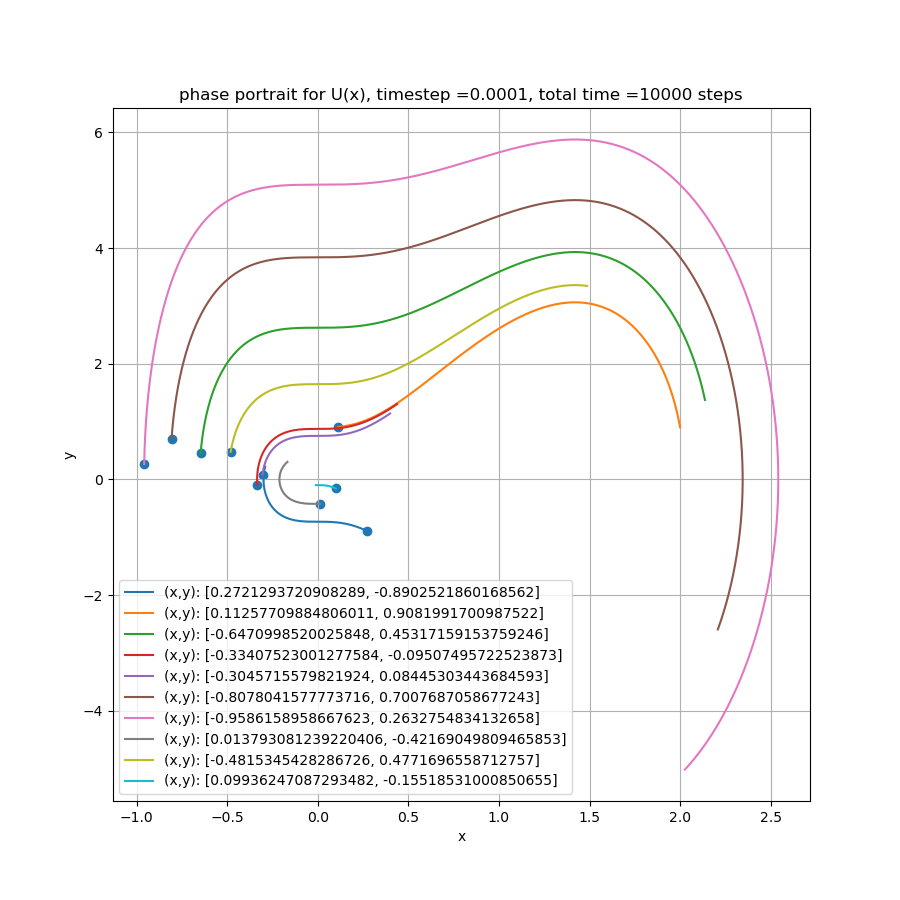
\includegraphics[width = 0.5 \textwidth]{mat461A1q310000 timesteps.png}$$
$$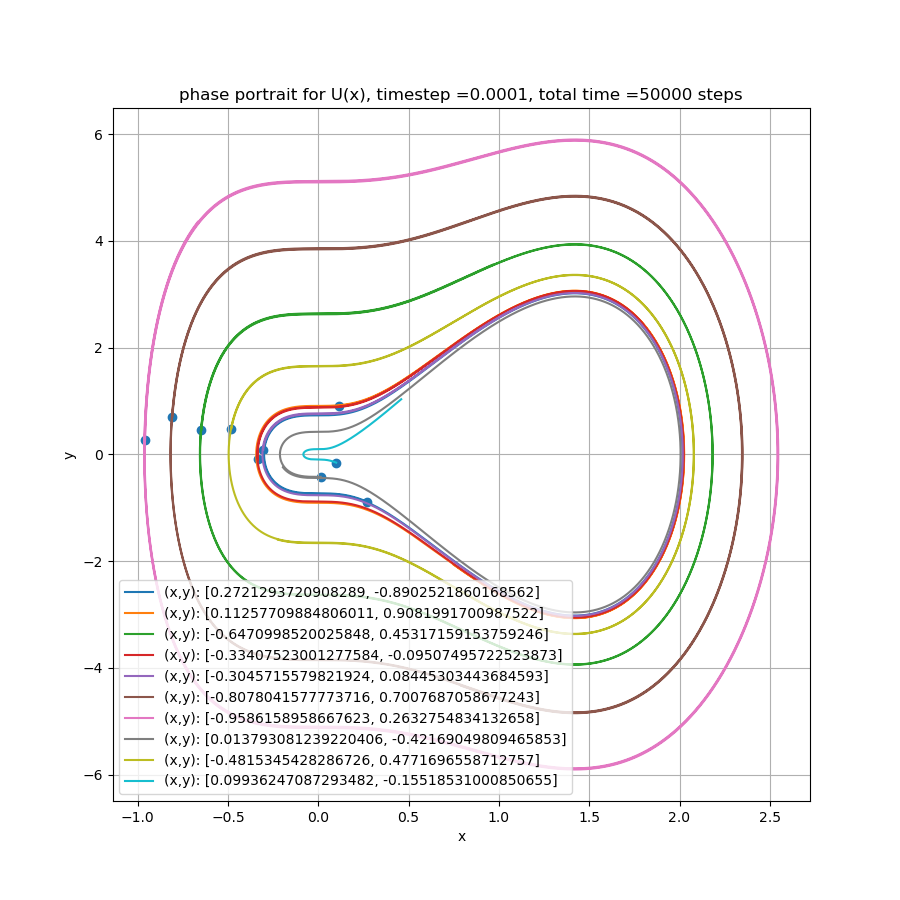
\includegraphics[width = 0.5 \textwidth]{mat461A1q350000 timesteps.png}$$
The paths taken by these particles behave as expected, matching the sketch given in $Q2$. 
The code used to generate these graphics is:
\begin{python}
	import numpy as np
	import matplotlib.pyplot as plt
	import random
	def potential_function(x):
	
	return -x**2*(x-2)*(x-4)
	
	def force(x):
	
	return x**2*(5*x**2-24*x+24)
	
	def vector_field(x_y_pair):
	
	return [x_y_pair[1] , force(x_y_pair[0])]
	
	def energy(x_y_pair):
	
	return 0.5*x_y_pair[1]**2  + potential_function(x_y_pair[0])
	
	
	def integrate_trajectory(initial_position, delta_t, time_steps):
	curve = []
	new_position = initial_position
	
	for i in range(time_steps):
	new_position = [new_position[j] + delta_t * vector_field(new_position)[j] for j in range(2)]
	curve.append(new_position)
	
	return curve
	
	delta_t = 0.0001
	time_steps = 10000
	initial_positions = []
	for i in range(10):
	x_rand = random.uniform(-1,1)
	y_rand = random.uniform(-1,1)
	initial_positions.append([x_rand,y_rand])
	plt.figure(figsize=(9, 9))
	print(initial_positions)
	
	initial_positions = [[0.2721293720908289, -0.8902521860168562], [0.11257709884806011, 0.9081991700987522], [-0.6470998520025848, 0.45317159153759246], [-0.33407523001277584, -0.09507495722523873], [-0.3045715579821924, 0.08445303443684593], [-0.8078041577773716, 0.7007687058677243], [-0.9586158958667623, 0.2632754834132658], [0.013793081239220406, -0.42169049809465853], [-0.4815345428286726, 0.4771696558712757], [0.09936247087293482, -0.15518531000850655]]
	
	
	for initial_position in initial_positions:
	curve = integrate_trajectory(initial_position, delta_t, time_steps)
	
	x_curve, y_curve = zip(*curve)
	
	plt.plot(x_curve, y_curve, label=f'(x,y): {initial_position}')
	
	initial_positions = np.array(initial_positions)
	plt.scatter(initial_positions[:, 0], initial_positions[:, 1])
	
	title = "mat461A1q3" + str(time_steps) + " timesteps.png"
	plt.xlabel('x')
	plt.ylabel('y')
	plt.title('phase portrait for U(x),' + ' timestep =' + str(delta_t ) + ', total time =' + str(time_steps) + ' steps')
	plt.legend()
	plt.grid(True)
	plt.savefig(title)
	plt.show()
\end{python}
Some issues encountered were with the range of points being generated. for points with $x$ component less than $-1$, they would diverge off to infinity very quickly. To make sure that the points in the given region did not diverge, a small time increment was chosen. To expand the region where points are generated, one could normalize the potential function with some constant so it diverges less quickly

\newpage
\begin{problem}
\end{problem}
Choose $x_1,x_2$ so that the time it takes to travel from $x_1$ to $x_2$ is half a period and corresponding $y$ values are $0$.  By Q5 the time it takes to get from $x_1$ to $x_2$ is $\int_{x_1}^{x_2} \frac{dx}{\sqrt{2(E-U(x))}}$. By symmetry a full period is $\int_{x_1}^{x_2} \frac{2}{\sqrt{2(E-U(x))}}dx =T$. 
We also have that 
$$T = \int_{x_1}^{x_2} \frac{2}{\sqrt{2(E-U(x))}}dx = \frac{d}{dE} 2\int_{x_1}^{x_2} \sqrt{2(E-U(x)}dx= \frac{d}{dE} 2\int_{x_1}^{x_2} ydx.$$
Since $2\int_{x_1}^{x_2} y dx$ is the area enclosed by $E$, we have that $\frac{dS(E)}{dE} = T$. 
\newpage
\begin{problem}
\end{problem}
We compute the integral $\int_{x_1}^{x_2} \frac{dx}{\sqrt{2(E-U(x))}}$ for $x_1 < x_2$. 
\begin{align*}
\int_{x_1}^{x_2} \frac{dx}{\sqrt{2(E-U(x))}}  & = \int_{x_1}^{x_2} \frac{dx}{\sqrt{2T}} \tag{Since $E = U(x) +T$ }
\\ & = \int_{x_1}^{x_2} \frac{dx}{\dot{x}} \tag{$T = \frac{1}{2}\dot{x}^2$}
\\ & = \int_{x_1}^{x_2} \frac{1}{\frac{dx}{dt}} dx
\\ & = \int_{x_1}^{x_2} \frac{dt}{dx} dx \tag{by inverse function theorem}
\\ & = t (x_2) - t(x_1) \tag{FTC}
\\ & = t_2-t_1
\end{align*}
The above formula is valid for any $x_1,x_2$ where $y_1,y_2$ both positive or both negative, so that we can apply the inverse function theorem. If $x_1>x_2$ choose the negative branch of the square root to get the same result. 
\newpage
\begin{problem}
\end{problem}
On $\Omega = \R^2 \setminus \{x>0, y \neq 0\}$, consider the potential $U(x,y) = \arctan \left(\frac{y}{x}\right)$. This is smooth on $\Omega$, so it makes sense to define it as a potential. We compute the gradient as 
$$-\grad U(x,y) = \bmat{-\frac{\partial U}{\partial x} & -\frac{\partial U}{ \partial y}} = \bmat{\frac{y}{x^2+y^2}  & -\frac{x}{x^2+y^2}}. $$
However on $\R^2 \setminus\{0\}$ this is not the case. $F$ being a conservative vector field is equivalent to the differential 1-form $\omega = \frac{y}{x^2+y^2} dx - \frac{x}{x^2+y^2}dy $ being exact on  $\R^2 \setminus \{0\}$. We show that this is not so by integrating along the closed $1-$chain $c:[0,2\pi] \to \R^2 \setminus\{0\}$ defined as $c(t) = (r\cos t, r \sin  t)$. We integrate in the usual way: 
$$\int_c \omega = \int_{[0,2\pi]} \frac{r\sin \theta}{r^2} \cdot -r\sin \theta d\theta - \frac{r\cos \theta}{r^2}\cdot r \cos \theta d\theta = \int_{[0,2\pi]} -1 d \theta  = -2\pi. $$
Therefore this form is not exact, and hence the vector field $F$ is not conservative. 
\end{document}
